\documentclass[a4paper,11pt,UTF8]{article}
\usepackage{ctex}
\usepackage{amsmath,amsthm,amssymb,amsfonts}
\usepackage{amsmath}
\usepackage[a4paper]{geometry}
\usepackage{graphicx}
\usepackage{microtype}
\usepackage{siunitx}
\usepackage{booktabs}
\usepackage[colorlinks=false, pdfborder={0 0 0}]{hyperref}
\usepackage{cleveref}
\usepackage{esint} 
\usepackage{graphicx}
\usepackage{ragged2e}
\usepackage{pifont}
\usepackage{extarrows}
\usepackage{mathptmx}
\usepackage{float}
\usepackage{caption}
\usepackage{subfigure}

\captionsetup[figure]{name={Figure}}

\title{Microelectronics Circuit Analysis and Design Homework(13rd)}
\author{Yuejin Xie \quad U202210333}
\date{Nov 3rd, 2023}
\begin{document}
\maketitle
1. Consider the feedback circuit in Figure 1.

\ding{172} Determine the feedback configuration and polarities, and you must label the instantaneous polarities in the figure.

\ding{173} Determine the effects of the feedback on the input resistor and the output resistor, and explain the output current or voltage tends to be stabilized.
\begin{figure}[H]
	\centering
	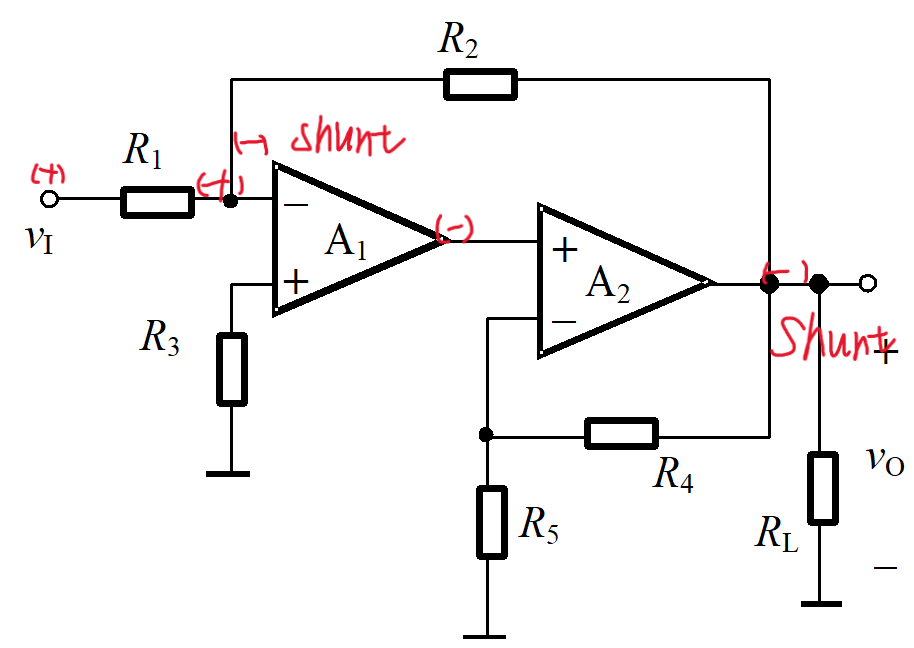
\includegraphics[width=0.5\textwidth]{12.1}
	\caption{Problem 1}
\end{figure}
2. The feedback circuits are shown in Figure 2. All capacitors act as short circuit to the sinusoidal signal.

\ding{172} Determine the feedback configuration and polarities, and you must label the instantaneous polarities in the figure.

\ding{173} Determine the effects of the feedback on the input resistor and the output resistor, and explain the output current or voltage tends to be stabilized
\begin{figure}[H]
	\subfigure[]{
		\centering
		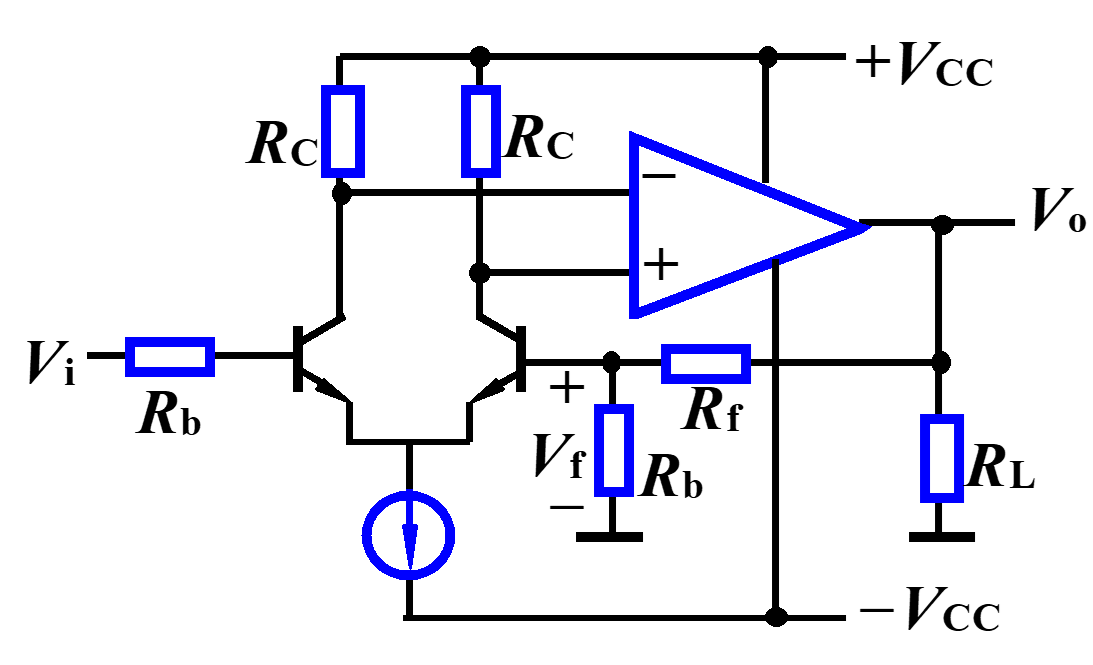
\includegraphics[width=0.3\textwidth]{12.2_1}

	}
	\subfigure[]{
		\centering
		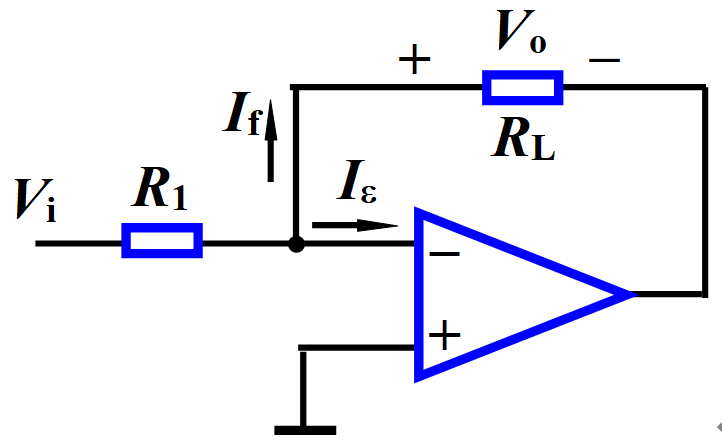
\includegraphics[width=0.3\textwidth]{12.2_2}

	}
	\subfigure[]{
		\centering
		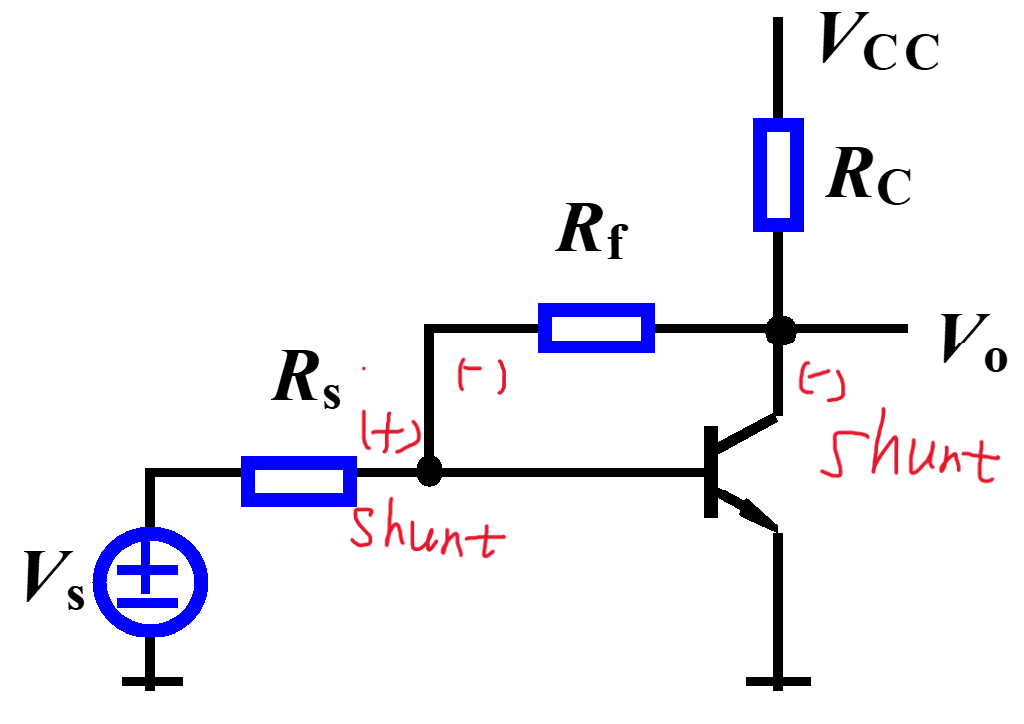
\includegraphics[width=0.3\textwidth]{12.2_3}

	}
	\caption{Problem 2}
\end{figure}
\end{document}